\newpage
\subsection{Problem 4 - Markowitz Portfolio Optimization}
\textbf{For a given return, R, formulate Markowitz’ Portfolio optimization problem as a quadratic program.}

The classical Markowitz objective function is given by
\begin{equation}
w^{T}\Sigma w-q*R^{T}w
\end{equation}

where $w$ is the vector of weights corresponding to proportion of the portfolio invested in each asset, $\Sigma$ is the covariance matrix of the assets, $q$ is a scaling parameter called risk-tolerance factor and $R$ is a vector of expected returns for the securities. Risk-tolerance of 0 corresponds to just minimizing the risk, i.e. the second part of the objective function can be left out. Changing the notation, this can be written as

\begin{equation}
\frac{1}{2} x'Hx
\end{equation}

There are two inequality constraints, one to specify the minimum required return and one to ensure that each of the portfolio weights is non-negative. If short-selling is allowed the later of these constraints can be removed. There is also a single equality constraint that ensures the weights of assets in the portfolio sum up to one, this makes the assumption that all of the available money is invested in this market. The quadratic program is thus

\begin{equation}
\begin{aligned}
    \min_{x} f(x) = \frac{1}{2} x'Hx \\
    s.t. \quad Ax \leq b \\
    -x_i \leq 0 \\
    A_{eq}x = 1
\end{aligned}
\end{equation}



\[H=2 \times \begin{bmatrix}
 	2.30 & 0.93 & 0.62 & 0.74 & -0.23 \\
   	0.93 & 1.40 & 0.22 & 0.56 & 0.26 \\
    0.62 & 0.22 & 1.80 & 0.78 & -0.27 \\
    0.74 & 0.56 & 0.78 & 3.40 & -0.56 \\
   	-0.23 & 0.26 & -0.27 & -0.56 & 2.60	
\end{bmatrix}
\]

\[A= \begin{bmatrix}
 	-15.10 & -12.50 & -14.70 & -9.02 & -17.68
\end{bmatrix}
\]

\[A_{eq}= \begin{bmatrix}
 	1 & 1 & 1 & 1 & 1 
\end{bmatrix}
\]

\[b=-10
\]

One could also include the inequality constraints on weights $x_i$ in the A matrix by means of a diagonal matrix where diagonal elements are all -1. In that case a vector of zeros would need to be appended to b as well. Additionally, the equality constraint could also be included in the same A matrix by adding rows of negative ones and positive ones to the matrix and corresponding -1 and 1 to the b vector. 

\textbf{What is the minimal and maximal possible return in this financial market?}

Maximal expected return is attained if the entire portfolio is just the single security with the highest return, which in this case is 17.68\%. Similarly, assuming short-sales are not allowed, the minimal expected return is 9.02\%. Assuming shorting with no additional costs is allowed, the minimal possible expected return is -17.68\%.

\textbf{Use quadprog to find a portfolio with return, R = 10.0, and minimal risk. What is the optimal portfolio and what is the risk (variance)?}

Setting the minimum required return to 10 yields the following portfolio weights and variance.

\[x'= \begin{bmatrix}
    0.0883 & 0.2509 & 0.2824 & 0.1038 & 0.2748
\end{bmatrix}
\]

\[\sigma^2 = 0.6249
\]

An important note is that the return of this portfolio is actually R = 14.4129. This means that there is no efficient portfolio with return 10. This portfolio is the minimum variance portfolio. One could also change the return constraint to an equality instead of inequality but in that case the portfolios yielded by the optimization routine would only be efficient if the return was set to above 14.4129. If exactly 10 percent expected return is desired, one should invest a portion of the money in some efficient portfolio (specifically, the portfolio which maximizes Sharpe ratio i.e. the tangency portfolio) and the rest into a zero return zero risk asset, that is withhold from investing it at all. 

\textbf{Compute the efficient frontier, i.e. the risk as function of the return. Plot the efficient frontier as well as the optimal portfolio as function of return.}

Figure \ref{fig:frontier_1} shows the efficient frontier as well as the minimum variance portfolio obtained in the previous step. 

As can be seen from the plot initially the return increases greatly as we take on slightly more risk than the minimum variance portfolio but above around 16.5\% return the effect slows down as the efficient portfolio approaches the security with the largest return and the risk reduction from diversification is lost.

\begin{figure}
    \centering
    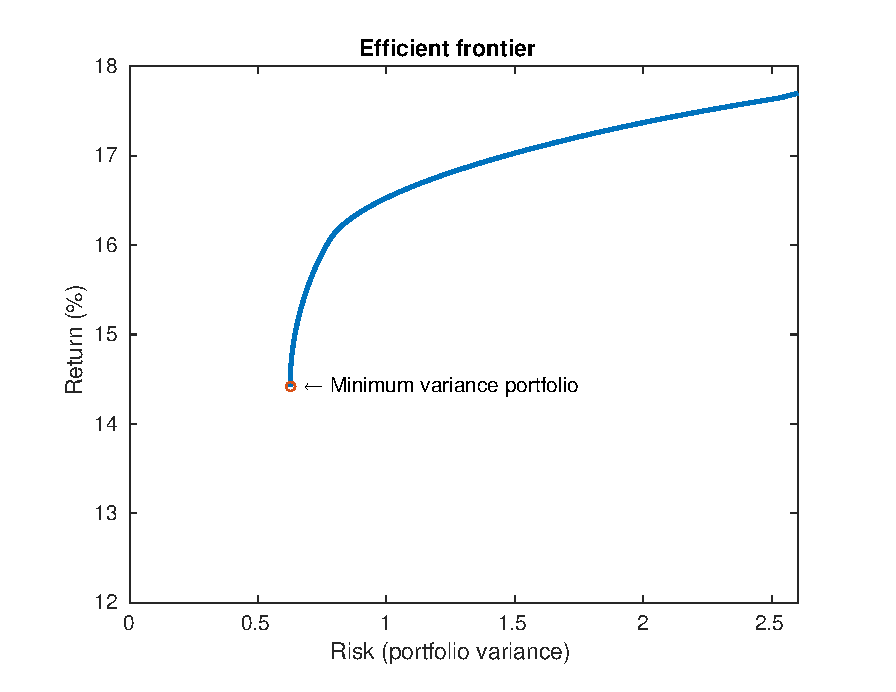
\includegraphics[width = 0.8\textwidth]{eff_front1.eps}
    \caption{Efficient frontier}
    \label{fig:frontier_1}
\end{figure}


\textbf{In the following we add a risk free security to the financial market. It has return $r_f = 2.0$. What is the new covariance matrix and return vector?}

Since there is no uncertainty in the return of the risk free asset and it is not related to the performance of the rest of the market, a row and column of zeros should be added to the covariance matrix. 

\[H=2 \times \begin{bmatrix}
 	2.30 & 0.93 & 0.62 & 0.74 & -0.23 & 0 \\
   	0.93 & 1.40 & 0.22 & 0.56 & 0.26  & 0 \\
    0.62 & 0.22 & 1.80 & 0.78 & -0.27 & 0\\
    0.74 & 0.56 & 0.78 & 3.40 & -0.56 & 0\\
   	-0.23 & 0.26 & -0.27 & -0.56 & 2.60 & 0	\\
   	0 & 0 & 0 & 0 & 0 & 0	\\
\end{bmatrix}
\]

\[returns'= \begin{bmatrix}
 	15.10 & 12.50 & 14.70 & 9.02 & 17.68 & 2.0
\end{bmatrix}
\]



\textbf{Compute the efficient frontier, plot it as well as the (return,risk) coordinates of all the securities. Comment on the effect of a risk free security. Plot the optimal portfolio as function of return.}

Figure \ref{fig:frontier_2} shows the two efficient frontiers as well as each of the 5 risky securities. With the risk free security one can have an efficient portfolio with arbitrary level of risk (up to 2.60 - the risk for largest return asset). Risk zero with the entire portfolio invested in the risk free asset and as a larger return is desired the proportion of portfolio in risk free security gradually decreases and the proportion in risky assets rises. Above around 15\% return the two efficient frontiers are essentially the same since to achieve these returns virtually nothing can be invested in the risk free security.

\begin{figure}
    \centering
    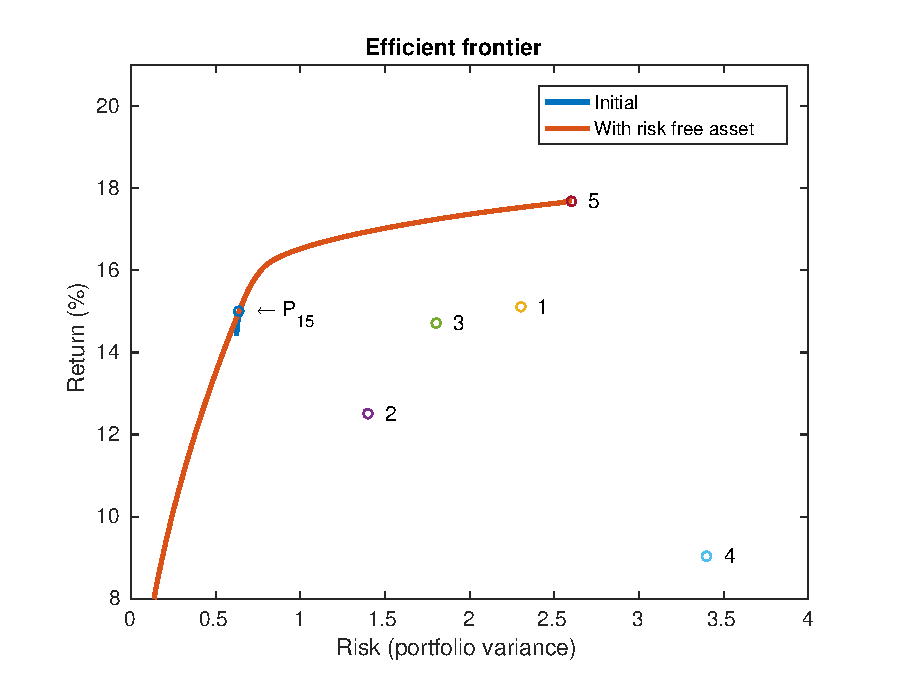
\includegraphics[width = 0.8\textwidth]{eff_front2.eps}
    \caption{Efficient frontier with risk free asset}
    \label{fig:frontier_2}
\end{figure}


\textbf{What is the minimal risk and optimal portfolio giving a return of R = 15.00. Plot this point in your optimal portfolio as function of return as well as on the efficient frontier diagram}

The weights and variance for optimal portfolio with R=15.00 are the following.

\[x'_{P_{15}}= \begin{bmatrix}
 	0.1655 & 0.1365 & 0.3115 & 0.0266 & 0.3352 & 0.0247
\end{bmatrix}
\]

\[\sigma_{P_{15}}^2 = 0.6249
\]

This portfolio can be seen on figure \ref{fig:frontier_2} ($P_{15}$)